\newpage

\section{Использованные данные}

\subsection{Теоретическое введение}

Тест Стернберга --- классический эксперимент, проведенный в 1966 году психологом
Солом Стернбергом, позволивший сделать вывод о том, что информация извлекается из
кратковременной памяти путём последовательного исчерпывающего сканирования.
Оригинальные и модифицированные схемы теста (Sternberg item recognition paradigm,
SIRP), описанного в статье \cite{Sternberg_item_recognition}, используются для изучения особенностей кратковременной и рабочей памяти. 

Оригинальный тест состоял из 24 тренировочных и 144 тестовых проб. В каждой пробе участнику эксперимента
предъявлялся произвольный набор цифр, который требовалось запомнить. Длина набора
варьировалась от 1 до 6 цифр, каждая из которых предъявлялась отдельно в течение 1-2 секунды.
После этого следовала пауза длиной в 2 секунды, а за ней контрольная цифра. Испытуемые должны
были потянуть один из двух рычагов в качестве ответа «Да, это одна из запомненных цифр» или «Нет,
это новая цифра» (требовавшиеся с одинаковой вероятностью), после чего контрольный стимул исчезал,
а загоравшаяся лампочка давала обратную связь о правильности ответа. В конце испытуемых также
просили произнести запомненную последовательность (схема экспериментальной установки изображена
на рис. \ref{fig_1}). \\[0.3 cm]
\textbf{Подробный сценарий каждого теста:}

\begin{enumerate}
    \item предупреждающий сигнал;
    \item запоминаемый стимул-образец;
    \item отсрочка;
    \item предупреждающий сигнал;
    \item контрольный стимул;
    \item ответ испытуемого;
    \item обратная связь о правильности выполнения задания;
    \item просьба к испытуемому вспомнить стимул-образец, после чего начинается следующая проба.
\end{enumerate}

\vspace*{10 mm}
\begin{figure}[H]
    \centering
    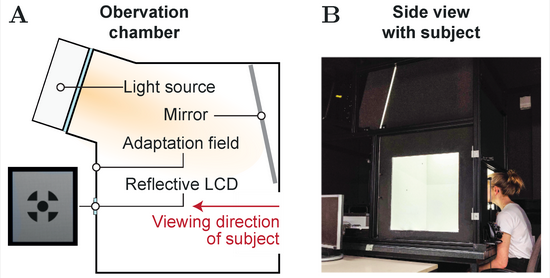
\includegraphics[width=0.6\linewidth]{images/1.png}
    \caption{Экспериментальная установка. (А) Схематическое изображение камеры наблюдения и
    направления обзора. (B) Изображение вида сбоку камеры наблюдения \cite{sternberg_paradigm}}
    \label{fig_1}
\end{figure}

\vspace*{5 mm}
Парадигма Стернберга была успешно использована в рамках изучения индивидуальных различий в
процессах памяти у здоровых участников \cite{paradigm_1}, \cite{paradigm_2}, в
исследованиях посвященных изучению дефицитарности и изменений кратковременной памяти при
старении \cite{paradigm_3}, в исследованиях шизофрении и болезни
Альцгеймера \cite{paradigm_4}, депрессии \cite{paradigm_5}, множественного склероза \cite{paradigm_6}, в
исследованиях изучающих воздействия различных медикаментов на процессы памяти \cite{paradigm_7}.\\[0.5 cm]

\subsection{Процедура снятия ЭЭГ данных}
\label{sec:chapter_2_2}

\vspace*{10 mm}
В настоящем исследования для получения ЭЭГ данных использовался "Тест Стернберга".
В эксперименте на голову участника исследования одевается специальная шапочка со специальными
металлическими электродами, которые регистрирует биоэлектрическую активность мозга (см. рис.
\ref{fig_2}). Каждый электрод с какой-то частотой (обычно 500-1000 Гц) регистрирует амплитуду
колебаний электромагнитной активности изменения электрического потенциала с поверхности головы. 

\begin{wrapfigure}{r}{0.4\textwidth}
    \centering
    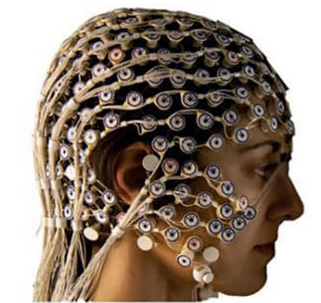
\includegraphics[width=0.4\textwidth]{images/2.png}
    \caption{Расположение электродов на поверхности головы}
    \label{fig_2}
\end{wrapfigure}

Затем участнику эксперимента последовательно предъявляются наборы цифр.
В каждом наборе цифры от 1 до 9 (без повторений одной цифры дважды) были представлены в случайной
последовательности. При этом размеры наборов могут отличаться (в оригинальных исследованиях
Стернберга, как было описано выше, это наборы объемом от 1 до 6 цифр). В зависимости от того,
какой длины последовательность была предъявлена участнику, определялся тип решаемой задачи:
лёгкая, средняя, повышенной сложности и тяжёлая (3, 4, 5 или 6 и более цифр для запоминания
соответственно) --- всего 4 типа задачи. Цифры показываются одна
за другой, участнику необходимо запомнить их последовательность. После контрольного сигнала
(появление определенной цифры на экране) участнику необходимо как можно быстрее ответить,
присутствовала ли цифра в предъявленном до этого наборе. После этого участника просят вспомнить
порядок представления цифр, для того чтобы убедиться, что он действительно запомнил
последовательность.

Перед предъявлением набора стимулов участникам эксперимента предъявляется фиксационный крест
на 1 секунду. Предъявление набора стимулов начинается через 1.2 секунды после предъявления
фиксационного креста и длится 1.5 секунды. Через 2 секунды после окончания предъявления набора
предъявляется тестовый стимул (задача участника - сказать был ли тестовый стимул в наборе).
Тестовый стимул предъявляется на 2 секунды. С момента начала предъявления тестового стимула
участник может давать ответ.

В исследовании принимал участие 101 человек. Каждому человеку предлагалось для решения порядка
30 задач на каждый из 4 типов.